% RESULTADOS-------------------------------------------------------------------

\chapter{CARACTERÍSTICAS MARCANTES}
\section{ANÁLISE LÉXICA}
De acordo com \citeonline{10.5555/2011965}, a análise léxica é uma análise do interpretador, os programas são lidos por um analisador sintático que divide o código em \textit{tokens}.
Todo programa é dividido em linhas lógicas que são separadas pelo \textit{token NEWLINE}, as linhas físicas são trechos de código divididos pelo caractere \textit{ENTER}.
Linhas lógicas não podem ultrapassar linhas físicas com exceção de junção de linhas, por exemplo:

\begin{algorithm}
    \caption{Exemplo do Interpretador Interativo}
    \textbf{if} resultado > 2 \textbf{and} 1 <= 5  \textbf{and} 2 < 5:\\
    \textbf{print}('Resultado: \%f' \% d)\\
ou\\
MESES COMO $= ['janeiro', 'fevereiro', 'março',$\\
                $'abril',   'maio',      'junho',$\\
               $ 'julho',   'agosto',    'setembro',$\\
                $'outubro', 'novembro',  'dezembro']$\\
\end{algorithm}


Para a delimitação de blocos de códigos, os delimitadores são colocados em uma pilha e diferenciados por sua indentação, iniciando a pilha com valor 0 (zero) e colocando valores maiores que os anteriores.
Para cada começo de linha, o nível de indentação é comparado com o valor do topo da pilha.
\begin{itemize}
    \item Se o número da linha for igual ao topo da pilha, a pilha não é alterada.
    \item Se o valor for maior, a pilha recebe o nível de indentação da linha e o nome \textit{INDENT (psuh)}.
    \item Se o nível de indentação for menor, então é desempilhado até chegar a um nível de indentação recebendo o nome \textit{DEDENT (pop)}.
    \item Se não encontrar nenhum valor, é gerado um erro de indentação.
\end{itemize}
\par Abaixo um exemplo de permutação, retirado do capítulo 2.1 sobre Estrutura de linhas na Análise léxica do Manual de Referência da linguagem\footnote{
    \citeonline[p. ~37]{10.5555/2011965}, vide figura \ref{fig:figura-ident-python}: p. \pageref{fig:figura-ident-python}, seção: ANÁLISE LÉXICA
}:

\begin{figure}[!htb]
    \centering
    \caption{Indentação em Python}
    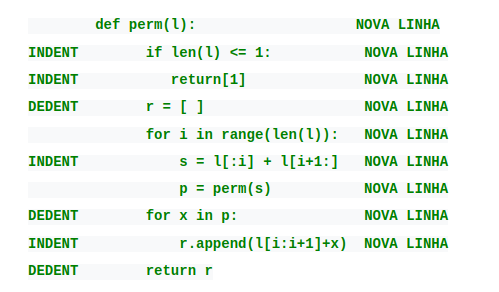
\includegraphics[width=0.75\textwidth]{./dados/figuras/ident1.png}
    \fonte{\citeonline{10.5555/2011965}}
    \label{fig:figura-ident-python}
\end{figure}

Python foi desenvolvido para ser uma linguagem de fácil leitura, com um visual agradável, frequentemente usando palavras e não pontuações como em outras linguagens.
Para a separação de blocos de código, a linguagem usa espaços em branco e indentação ao invés de delimitadores visuais como chaves (C, Java) ou palavras (BASIC, Fortran, Pascal).
Diferente de linguagens com delimitadores visuais de blocos, em Python a indentação é obrigatória.
O aumento da indentação indica o início de um novo bloco, que termina da diminuição da indentação.
\par Usando um editor de texto comum é muito fácil existirem erros de indentação, o recomendado é configurar o editor conforme a análise léxica do Python ou utilizar uma IDE.
Todas as IDE que suportam a linguagem fazem indentação automaticamente.\\    
Exemplo:

\begin{figure}[!htb]
    \centering
    \caption{Indentação em Python}
    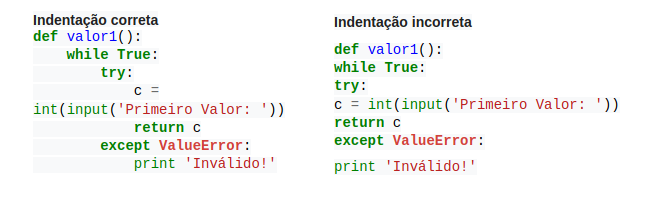
\includegraphics[width=0.75\textwidth]{./dados/figuras/ident2.png}
    \fonte{\citeonline{10.5555/2011965}}
    \label{fig:figura-ident2-python}
\end{figure}

O analisador léxico reconhecerá as palavras reservadas while, def, try, except, return, print e as cadeias de caracteres entre aspas simples e a indentação, e se não houver problemas o programa executará normalmente, senão apresentará a exceção: \textit{IndentationError\footnote{
    \citeonline[p. ~20]{pyMan}
}}.

\section{COMPILADOR DE BYTECODE}
A linguagem é de altíssimo nível, como já dito, mas ela também pode compilar seus programas para que a próxima vez que o executar não precise compilar o novamente, reduzindo o tempo de carga na execução.
\par Utilizando o interpretador interativo não é necessário a criação do arquivo de Python compilado, os comandos são executados interativamente.
Entretanto, quando um programa ou um módulo é evocado, o interpretador realiza a análise léxica e sintática, compila o código de alto nível se necessário e o executa na máquina virtual da linguagem.
\par O bytecode é armazenado em arquivos com extensão \textit{.pyc ou .pyo}, este último no caso de bytecode otimizado\footnote{
    Interessante notar que o bytecode da linguagem também é de alto nível, ou seja, é mais legível aos seres humanos que o código de byte do C, por exemplo.}.
\par Normalmente, o Python trabalha com dois grupos de arquivos:

\begin{itemize}
    \item Os módulos do núcleo da linguagem, sua biblioteca padrão e os módulos independentes, criados pelo usuário.
    \item No núcleo do interpretador existe o analisador léxico, o analisador sintático que utiliza Estruturas de Objetos (tempo de execução), o Compilador que aloca memória (tempo de execução) e depois do Avaliador de código que modifica o estado atual do programa (tempo de execução), mostrando resultado para o usuário.
\end{itemize}

\section{ORIENTAÇÃO A OBJETO}
Python suporta a maioria das técnicas da programação orientada a objeto.
Qualquer objeto pode ser usado para qualquer tipo, e o código funcionará enquanto haja métodos e atributos adequados.
O conceito de objeto na linguagem é bastante abrangente: classes, funções, números e módulos são todos considerados objetos.
Também há suporte para metaclasses, polimorfismo, e herança (inclusive herança múltipla).
Há um suporte limitado para variáveis privadas.

\par Na versão 2.2 de Python foi introduzido um novo estilo de classes em que objetos e tipos foram unificados, permitindo a especialização de tipos.
Já a partir da versão 2.3 foi introduzido um novo método de resolução de ambiguidades para heranças múltiplas.\cite{30}

Uma classe é definida com \textit{class} nome, e o código seguinte é a composição dos atributos.
Todos os métodos da classe recebem uma referência a uma instância da própria classe como seu primeiro argumento, e a convenção é que se chame este argumento self.
Assim os métodos são chamados objeto.método(argumento1, argumento2) e são definidos iguais a uma função, como método(self, argumento1, argumento2).
Veja que o parâmetro self conterá uma referência para a instância da classe definida em objeto quando for efetuada esta chamada.
Os atributos da classe podem ser acessados em qualquer lugar da classe, e os atributos de instância (ou variável de instância) devem ser declarados dentro dos métodos utilizando a referência à instância atual (self)

Em Python não existe proteção dos membros duma classe ou instância pelo interpretador, o chamado encapsulamento.
Convenciona-se que atributos com o nome começando com um são de uso privado da classe, mas não há um policiamento do interpretador contra acesso a estes atributos.
Uma exceção são nomes começando com, no caso em que o interpretador modifica o nome do atributo.

\par Python permite polimorfismo, que condiz com a reutilização de código.
É fato que funções semelhantes em várias partes do software sejam utilizadas várias vezes, então definimos esta função como uma biblioteca e todas as outras funções que precisarem desta a chamam sem a necessidade de reescrevê-la.

\par Python não possui overloading; não é possível criar duas funções com o mesmo nome, pois elas são consideradas atributos da classe.
Caso o nome da função se repita em outra assinatura, o interpretador considera esta última como override e sobrescreve a função anterior.
Algumas operações entre diferentes tipos são realizadas através de coerção ($ex.: 3.2 + 3$).

\par É possível encapsular abstrações em módulos e pacotes. Quando um arquivo é criado com a extensão \textit{.py}, ele automaticamente define um módulo.
Um diretório com vários módulos é chamado de pacote e deve conter um modulo chamado $\_\_init\_\_$, para defini-lo como principal.
Estas diferenciações ocorrem apenas no sistema de arquivos. Os objetos criados são sempre módulos.
Caso o código não defina qual dos módulos será importado, o padrão é o $\_\_init\_\_$.

\section{PROGRAMAÇÃO FUNCIONAL}
Uma das construções funcionais de Python é a compreensão de listas\footnote{
    Compreensão de lista é uma construção sintática disponível em algumas linguagens de programação para criação de uma lista baseada em listas existentes.
    Ela segue a forma da notação de definição de conjunto matemática (compreensão de conjunto) como forma distinta para uso de funções de mapa e filtro. \citeonline{list}
}, uma forma eficiente de construir listas.
Por exemplo, pode-se usar a técnica para calcular as cinco primeiras potências de dois.
O algoritmo quicksort também pode ser expresso usando a mesma técnica.

Em Python, funções são objetos de primeira classe que podem ser criados e armazenados dinamicamente.
O suporte a funções anônimas está na construção lambda (Cálculo-$\lambda$).
Não há disponibilidade de funções anônimas de fato, pois os lambdas contêm somente expressões e não blocos de código.

Python também suporta clausuras léxicas desde a versão 2.2.
Já geradores foram introduzidos na versão 2.2 e finalizados na versão 2.3, e representam o mecanismo de Python para a avaliação preguiçosa\footnote{
    Avaliação preguiçosa (também conhecida por avaliação atrasada) é uma técnica usada em programação para atrasar a computação até um ponto em que o resultado da computação é considerado suficiente, o necessário.
Os benefícios da avaliação preguiçosa incluem o aumento do desempenho ao evitar cálculos desnecessários, evitando condições de erro na avaliação de expressões compostas, a habilidade em construir estruturas de dados infinitas e a habilidade de definir estruturas do controle como funções regulares melhor que usando primitivas internas.
No oposto de avaliação atrasada está avaliação ansiosa, também conhecido como avaliação rigorosa. \citeonline{pldc}
} de funções. 


\section{TRATAMENTO DE EXCEÇÕES}

Python suporta e faz uso constante de tratamento de exceções como uma forma de testar condições de erro e outros eventos inesperados no programa.
É inclusive possível capturar uma exceção causada por um erro de sintaxe.
O estilo da linguagem apoia o uso de exceções sempre que uma condição de erro pode aparecer.
Por exemplo, ao invés de testar a disponibilidade de acesso a um recurso, a convenção é simplesmente tentar usar o recurso e capturar a exceção caso o acesso seja rejeitado.

\par Exceções são usadas frequentemente como uma estrutura de seleção, substituindo blocos \textit{if-else}, especialmente em situações que envolvem threads.
Uma convenção de codificação é o EAFP, do inglês, “é mais fácil pedir perdão que permissão”.
Isso significa que, em relação a desempenho, é preferível capturar exceções do que testar atributos antes de os usar.
Segue abaixo exemplos de código que testam atributos e que capturam exceções:

\begin{figure}[!htb]
    \centering
    \caption{Mount Python’s Logo}
    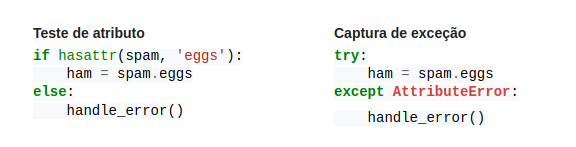
\includegraphics[width=1\textwidth]{./dados/figuras/tryCatch.png}
    \fonte{\citeonline{10.5555/2011965}}
    \label{fig:figura-mountPython}
\end{figure}

\par Ambos os códigos produzem o mesmo efeito, mas há diferenças de desempenho.
Quando spam possui o atributo eggs, o código que captura exceções é mais rápido.
Caso contrário, a captura da exceção representa uma perda considerável de desempenho, e o código que testa o atributo é mais rápido.
Geralmente, o paradigma da captura de exceções é mais rápido, e também pode evitar problemas de concorrência.
Por exemplo, num ambiente multitarefa, o espaço de tempo entre o teste do atributo e seu uso de fato pode invalidar o atributo, problema que não acontece no caso da captura de exceções.

\section{BIBLIOTECA PADRÃO}
Python possui uma grande biblioteca padrão\footnote{
    Algumas partes da biblioteca são cobertas por especificações (por exemplo, a implementação WSGI da wsgiref segue o PEP 333), mas a maioria dos módulos não o segue.
}, geralmente citada como um dos maiores trunfos da linguagem, fornecendo ferramentas para diversas tarefas.
Por conta da grande variedade de ferramentas fornecida pela biblioteca padrão, combinada com a habilidade de usar linguagens de nível mais baixo como C e C++, Python pode ser poderosa para conectar componentes diversos de software.

A biblioteca padrão conta com facilidades para escrever aplicações para a Internet, contando com diversos formatos e protocolos como MIME e HTTP.
Também há módulos para criar interfaces gráficas, conectar em bancos de dados relacionais e manipular expressões regulares.

\section{INTEROPERABILIDADE}
Outro ponto forte da linguagem é sua capacidade de interoperar com várias outras linguagens, principalmente código nativo.
A documentação da linguagem inclui exemplos de como usar a Python C-API para escrever funções em C\footnote{
    Mas atualmente esse \textit{sequer} é o modo mais indicado de interoperação, havendo alternativas tais como Cython, Swig ou cffi
} que podem ser chamadas diretamente de código Python.
A biblioteca Boost do C++ inclui uma biblioteca para permitir a interoperabilidade entre às duas linguagens, e pacotes científicos usam bibliotecas de alto desempenho numérico escritos em Fortran e mantidos há décadas.

\section{COMENTÁRIOS}
Python fornece duas alternativas para documentar o código.
A primeira é o uso de comentários para indicar o que certo código faz.
Comentários começam com \# e são terminados pela quebra da linha.
Não há suporte para comentários que se estendem por mais de uma linha; cada linha consecutiva de comentário deve indicar \#.
A segunda alternativa é o uso de cadeias de caractere, literais de texto inseridos no código sem atribuição.
Cadeias de caracteres em Python são delimitadas por $"$ ou $'$ para única linha e por $"""$ ou $'''$ para múltiplas linhas.
Entretanto, é convenção usar os métodos de múltiplas linhas em ambos os casos.

Diferente de comentários, as cadeias de caracteres usadas como documentação são objetos Python e fazem parte do código interpretado.
Isso significa que um programa pode acessar sua própria documentação e manipular a informação.
Há ferramentas que extraem automaticamente essa documentação para a geração da documentação de API a partir do código.
Documentação através de cadeias de caracteres também pode ser acessada a partir do interpretador através da função \textit{help()}.